% =====================================================================
%  Exercise Sheet Template  (compile with XeLaTeX or LuaLaTeX)
%  Layout: Part -> worked Example (numbered steps + dotted connectors)
%          -> Practice Questions (1 or 2 columns, optional visual models)
% =====================================================================
\documentclass{article}
\usepackage[margin=0.75in]{geometry}
\usepackage{xcolor}
\usepackage{amsmath}
\usepackage{amssymb}
\usepackage{fontspec}
\usepackage{tikz}
\usetikzlibrary{tikzmark, arrows.meta, positioning, decorations.pathreplacing, calc}
\usepackage{enumitem}
\usepackage{multicol}

% ---------------------------------------------------------------------
%  THEME & COLORS
% ---------------------------------------------------------------------
\definecolor{bglight}{HTML}{FFFFFF}
\definecolor{textlight}{HTML}{000000}
\definecolor{subtext}{HTML}{666666}

% Model colors
\colorlet{redbar}{red!70!black}
\colorlet{bluebar}{blue!55!black}
\colorlet{greenbar}{green!60!black}
\colorlet{yellowbar}{yellow!80!black}

\pagecolor{bglight}
\color{textlight}
\pagestyle{empty}

% ---------------------------------------------------------------------
%  BUILDING BLOCKS
% ---------------------------------------------------------------------

% Circled step number.  \stepnum{number}{node-name}
\newcommand{\stepnum}[2]{%
  \tikzmarknode{#2}{%
    \begin{tikzpicture}[baseline=(char.base)]
      \node[draw=textlight, circle, inner sep=1.5pt, font=\sffamily\small] (char) {#1};
    \end{tikzpicture}%
  }%
}

% Dotted connectors between consecutive step nodes.
\newcommand{\stepchain}[1]{%
  \begin{tikzpicture}[remember picture, overlay]
    \def\prevnode{}%
    \foreach \n in {#1} {%
      \ifx\prevnode\empty\else
        \draw[dotted, thick, textlight!60] (\prevnode.south) -- (\n.north);%
      \fi
      \xdef\prevnode{\n}%
    }%
  \end{tikzpicture}%
}

% Worked-example steps
\newenvironment{steps}{\begin{description}[leftmargin=2em]}{\end{description}}

% Practice questions
\newenvironment{questions}[1][1]{%
  \begin{enumerate}[label=\textbf{\arabic*.}, start=#1, itemsep=2em, leftmargin=2em]%
}{\end{enumerate}}

% Headings
\newcommand{\examplehead}[1]{{\Large \textbf{Example: #1}}\par\vspace{0.5em}}
\newcommand{\practicehead}[1]{%
  \vspace{1em}\noindent\textcolor{subtext!40}{\rule{\linewidth}{0.5pt}}\vspace{1.5em}\par
  {\Large \textbf{#1}}\par\vspace{1em}}

% Answer blanks
\newcommand{\blank}[1][1.5cm]{\underline{\hspace{#1}}}
\newcommand{\ans}[1]{{\color{subtext}#1}}

\newcommand{\working}[2]{%
  $\begin{aligned}[t] #1 &= \blank[3cm] \\ &= \blank[3cm] \\ &\vphantom{#2}\end{aligned}$}

% ---------------------------------------------------------------------
%  BAR-MODEL HELPERS  (use inside tikzpicture)
% ---------------------------------------------------------------------
\newcommand{\bbar}[5]{%
  \draw[fill=#4, draw=black, line width=0.5pt] (#1,#3) rectangle (#2,{#3+0.5});
  \node[font=\small, text=white] at ({(#1+#2)/2},{#3+0.25}) {#5};}
\newcommand{\topbrace}[4]{%
  \draw[decorate, decoration={brace, amplitude=4pt}, line width=0.5pt] (#1,#3) -- (#2,#3);
  \node[anchor=south, font=\small] at ({(#1+#2)/2},{#3+0.1}) {#4};}
\newcommand{\botbrace}[4]{%
  \draw[decorate, decoration={brace, amplitude=4pt, mirror}, line width=0.5pt] (#1,#3) -- (#2,#3);
  \node[anchor=north, font=\small] at ({(#1+#2)/2},{#3-0.1}) {#4};}

% ---------------------------------------------------------------------
%  BASE-10 BLOCK HELPERS (Flats = Hundreds, Rods = Tens, Units = Ones)
% ---------------------------------------------------------------------
% \bflat{x}{y}  Draws a 100-flat (1.5cm x 1.5cm grid)
\newcommand{\bflat}[2]{%
  \draw[fill=redbar!15, draw=black, line width=0.4pt] (#1,#2) rectangle ++(1.5,1.5);
  \foreach \i in {1,...,9} {
    \draw[line width=0.2pt, subtext!40] (#1+\i*0.15,#2) -- ++(0,1.5);
    \draw[line width=0.2pt, subtext!40] (#1,#2+\i*0.15) -- ++(1.5,0);
  }%
}
% \brod{x}{y}   Draws a 10-rod (0.15cm x 1.5cm rod)
\newcommand{\brod}[2]{%
  \draw[fill=bluebar!25, draw=black, line width=0.4pt] (#1,#2) rectangle ++(0.15,1.5);
  \foreach \y in {1,...,9} {
    \draw[line width=0.2pt, subtext!40] (#1,#2+\y*0.15) -- ++(0.15,0);
  }%
}
% \bunit{x}{y}  Draws a 1-unit cube (0.15cm x 0.15cm)
\newcommand{\bunit}[2]{%
  \draw[fill=yellowbar!60, draw=black, line width=0.4pt] (#1,#2) rectangle ++(0.15,0.15);
}

% =====================================================================
\begin{document}
\sffamily

% ================= HEADER =================
\begin{center}
  {\Huge \bfseries Introduction to SG Math} \\[0.4em]
  {\Large \textcolor{subtext}{Base-Ten Blocks, Bar Models \& Mental Math Strategies}}
\end{center}
\vspace{1em}

% =====================================================================
%  PART 1 -- Base-10 Addition Worked Example
% =====================================================================
\section*{Part 1: Base-10 Block Addition}

\noindent\textbf{Example:} Solve \textbf{$134 + 123$} using Hundreds (Flats), Tens (Rods), and Ones (Units).
\vspace{0.8em}

\begin{steps}
  \item[\stepnum{1}{p2s1}] \textbf{Represent each number using blocks}\\[0.4em]
  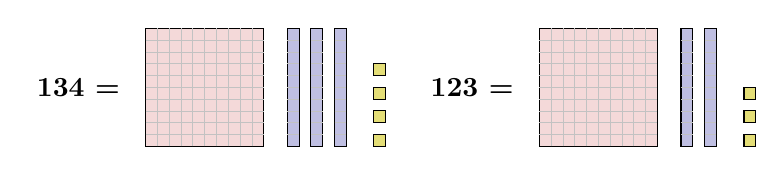
\begin{tikzpicture}[baseline={(0,0.75)}]
    % Number 134
    \node[anchor=east, font=\bfseries] at (1.0,0.85) {134 =};
    \bflat{1.2}{0.1}
    \brod{3.0}{0.1} \brod{3.3}{0.1} \brod{3.6}{0.1}
    \bunit{4.1}{0.1} \bunit{4.1}{0.4} \bunit{4.1}{0.7} \bunit{4.1}{1.0}

    % Number 123
    \node[anchor=east, font=\bfseries] at (6.0,0.85) {123 =};
    \bflat{6.2}{0.1}
    \brod{8.0}{0.1} \brod{8.3}{0.1}
    \bunit{8.8}{0.1} \bunit{8.8}{0.4} \bunit{8.8}{0.7}
  \end{tikzpicture}
  \vspace{0.6em}

  \item[\stepnum{2}{p2s2}] \textbf{Group hundreds, tens, and ones together}\\[0.4em]
  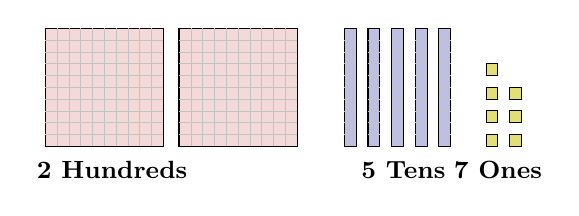
\begin{tikzpicture}[baseline={(0,0.8)}]
    % Combined
    \bflat{0}{0} \bflat{1.7}{0}
    \node[font=\small\bfseries] at (0.85,-0.3) {2 Hundreds};

    \brod{3.8}{0} \brod{4.1}{0} \brod{4.4}{0} \brod{4.7}{0} \brod{5.0}{0}
    \node[font=\small\bfseries] at (4.55,-0.3) {5 Tens};

    \bunit{5.6}{0} \bunit{5.6}{0.3} \bunit{5.6}{0.6} \bunit{5.6}{0.9} 
    \bunit{5.9}{0} \bunit{5.9}{0.3} \bunit{5.9}{0.6}
    \node[font=\small\bfseries] at (5.75,-0.3) {7 Ones};
  \end{tikzpicture}
  \vspace{1em}

  \item[\stepnum{3}{p2s3}] \textbf{Write the final value}\\[0.4em]
  \[ 2\text{ Hundreds} + 5\text{ Tens} + 7\text{ Ones} = 200 + 50 + 7 = \mathbf{257} \]
\end{steps}
\stepchain{p2s1,p2s2,p2s3}

\practicehead{Practice Questions}

\begin{questions}
  % Question 1: Reading Blocks
  \item \textbf{What total number is shown by the blocks below?}

  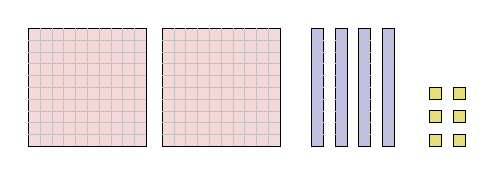
\begin{tikzpicture}[baseline={(0,0.5)}]
    \bflat{0}{0} \bflat{1.7}{0}
    \brod{3.6}{0} \brod{3.9}{0} \brod{4.2}{0} \brod{4.5}{0}
    \bunit{5.1}{0} \bunit{5.1}{0.3} \bunit{5.1}{0.6}
    \bunit{5.4}{0} \bunit{5.4}{0.3} \bunit{5.4}{0.6}
  \end{tikzpicture}

  \vspace{0.5em}
  $\blank\text{ Hundreds} + \blank\text{ Tens} + \blank\text{ Ones} = \blank$

  % Question 2: Addition with blocks
  \item \textbf{Add the blocks to find $142 + 115$:}

  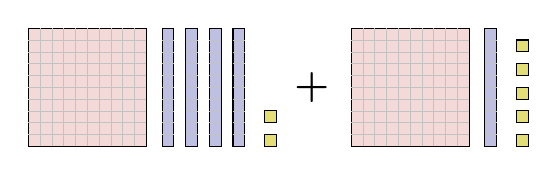
\begin{tikzpicture}[baseline={(0,0.5)}]
    % 142
    \bflat{0}{0}
    \brod{1.7}{0} \brod{2.0}{0} \brod{2.3}{0} \brod{2.6}{0}
    \bunit{3.0}{0} \bunit{3.0}{0.3}
    
    \node[font=\Large\bfseries] at (3.6,0.75) {+};

    % 115
    \bflat{4.1}{0}
    \brod{5.8}{0}
    \bunit{6.2}{0} \bunit{6.2}{0.3} \bunit{6.2}{0.6} \bunit{6.2}{0.9} \bunit{6.2}{1.2}
  \end{tikzpicture}

  \vspace{0.6em}
  Total $= \blank\text{ Hundreds} + \blank\text{ Tens} + \blank\text{ Ones} = \blank$
\end{questions}

\pagebreak

% =====================================================================
%  PART 2 -- Subtraction with Regrouping / Crossing Out
% =====================================================================
\section*{Part 2: Base-10 Subtraction (Taking Away)}

\noindent\textbf{Example:} Solve \textbf{$245 - 123$} by crossing out blocks.
\vspace{0.8em}

\begin{steps}
  \item[\stepnum{1}{p3s1}] \textbf{Build the starting number ($245$)}\\[0.4em]
  Start with 2 Hundreds, 4 Tens, and 5 Ones.
  \vspace{0.4em}

  \item[\stepnum{2}{p3s2}] \textbf{Take away $123$ (1 Hundred, 2 Tens, 3 Ones)}\\[0.4em]
  Cross out the subtracted amounts with red lines:
  \\[0.6em]
  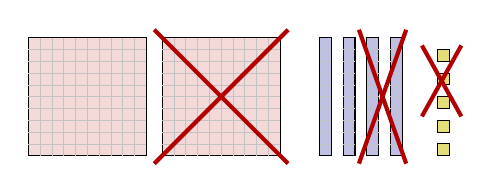
\begin{tikzpicture}[baseline={(0,0.5)}]
    % 2 Hundreds (1 crossed out)
    \bflat{0}{0}
    \bflat{1.7}{0}
    \draw[redbar, line width=1.5pt] (1.6,-0.1) -- (3.3,1.6);
    \draw[redbar, line width=1.5pt] (1.6,1.6) -- (3.3,-0.1);

    % 4 Tens (2 crossed out)
    \brod{3.7}{0} \brod{4.0}{0}
    \brod{4.3}{0} \brod{4.6}{0}
    \draw[redbar, line width=1.5pt] (4.2,-0.1) -- (4.8,1.6);
    \draw[redbar, line width=1.5pt] (4.2,1.6) -- (4.8,-0.1);

    % 5 Ones (3 crossed out)
    \bunit{5.2}{0} \bunit{5.2}{0.3}
    \bunit{5.2}{0.6} \bunit{5.2}{0.9} \bunit{5.2}{1.2}
    \draw[redbar, line width=1.5pt] (5.0,0.5) -- (5.5,1.4);
    \draw[redbar, line width=1.5pt] (5.0,1.4) -- (5.5,0.5);
  \end{tikzpicture}
  \vspace{0.6em}

  \item[\stepnum{3}{p3s3}] \textbf{Count remaining blocks}\\[0.2em]
  Remaining $= 1\text{ Hundred}, 2\text{ Tens}, 2\text{ Ones}$ \\[0.2em]
  \[ 245 - 123 = \mathbf{122} \]
\end{steps}
\stepchain{p3s1,p3s2,p3s3}

\practicehead{Practice Questions}

\begin{questions}
  % Question 1: Subtraction with crossing out
  \item \textbf{Cross out blocks to solve $236 - 114$:}

  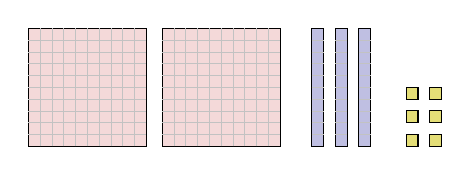
\begin{tikzpicture}[baseline={(0,0.5)}]
    \bflat{0}{0} \bflat{1.7}{0}
    \brod{3.6}{0} \brod{3.9}{0} \brod{4.2}{0}
    \bunit{4.8}{0} \bunit{4.8}{0.3} \bunit{4.8}{0.6}
    \bunit{5.1}{0} \bunit{5.1}{0.3} \bunit{5.1}{0.6}
  \end{tikzpicture}

  \vspace{0.6em}
  Remaining: $\blank\text{ Hundreds} + \blank\text{ Tens} + \blank\text{ Ones} = \blank$

  % Question 2: Regrouping concept
  \item \textbf{Regrouping Tens to Ones: $132 - 115$}
  
  \textit{Hint: Trade 1 Ten Rod for 10 Unit Cubes first, then take away 5 ones.}

  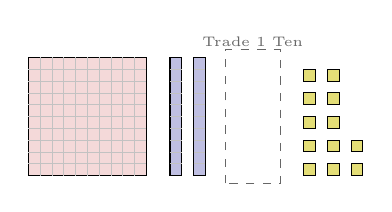
\begin{tikzpicture}[baseline={(0,0.5)}]
    \bflat{0}{0}
    \brod{1.8}{0} \brod{2.1}{0}
    % Traded Rod replaced by 10 units
    \draw[dashed, draw=subtext] (2.5,-0.1) rectangle (3.2,1.6);
    \node[font=\tiny, text=subtext] at (2.85,1.7) {Trade 1 Ten};
    
    % 2 original ones + 10 traded ones
    \bunit{3.5}{0} \bunit{3.5}{0.3} \bunit{3.5}{0.6} \bunit{3.5}{0.9} \bunit{3.5}{1.2}
    \bunit{3.8}{0} \bunit{3.8}{0.3} \bunit{3.8}{0.6} \bunit{3.8}{0.9} \bunit{3.8}{1.2}
    \bunit{4.1}{0} \bunit{4.1}{0.3}
  \end{tikzpicture}

  \vspace{0.6em}
  Equation: $132 - 115 = \blank$
\end{questions}

\pagebreak

% =====================================================================
%  PART 3 -- Bar Models
% =====================================================================
\section*{Part 3: Bar Models}

\noindent\textbf{Example:} Maya has \textbf{5 red pencils} and \textbf{3 blue pencils}.
How many pencils in total?
\vspace{0.8em}

\begin{steps}
  \item[\stepnum{1}{p1s1}] \textbf{Identify the parts}\\[0.2em]
  \begin{itemize}
    \item Red pencils $= 5$
    \item Blue pencils $= 3$
  \end{itemize}
  \vspace{0.6em}

  \item[\stepnum{2}{p1s2}] \textbf{Draw the bars}\\[0.6em]
  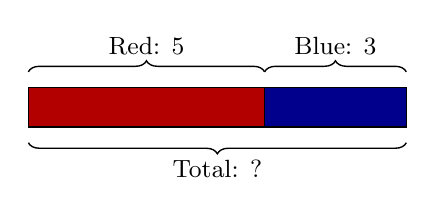
\begin{tikzpicture}[>=Stealth, baseline={(0,1.2)}]
    \topbrace{0}{3}{1.8}{Red: 5}
    \topbrace{3}{4.8}{1.8}{Blue: 3}
    \bbar{0}{3}{1.1}{redbar}{}
    \bbar{3}{4.8}{1.1}{bluebar}{}
    \botbrace{0}{4.8}{0.9}{Total: ?}
  \end{tikzpicture}
  \vspace{0.6em}

  \item[\stepnum{3}{p1s3}] \textbf{Write and solve}\\[0.4em]
  \[ 5 + 3 = \mathbf{8} \]
\end{steps}
\stepchain{p1s1,p1s2,p1s3}

\practicehead{Practice Questions}

\begin{questions}
  % Part-Whole Model
  \item \textbf{Lucas saved \$45 in January and \$38 in February. How much in total?}

  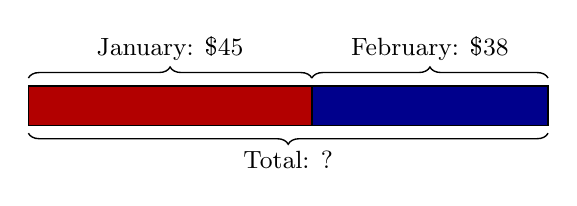
\begin{tikzpicture}[>=Stealth, baseline={(0,0.5)}]
    \topbrace{0}{3.6}{1.2}{January: \$45}
    \topbrace{3.6}{6.6}{1.2}{February: \$38}
    \bbar{0}{3.6}{0.6}{redbar}{}
    \bbar{3.6}{6.6}{0.6}{bluebar}{}
    \botbrace{0}{6.6}{0.5}{Total: ?}
  \end{tikzpicture}

  \vspace{0.5em}
  Equation: $\blank + \blank = \blank$ \hspace{2cm} Total = \$\blank

  % Comparison Model
  \item \textbf{Liam has 84 stamps, 26 more than Noah. How many does Noah have?}

  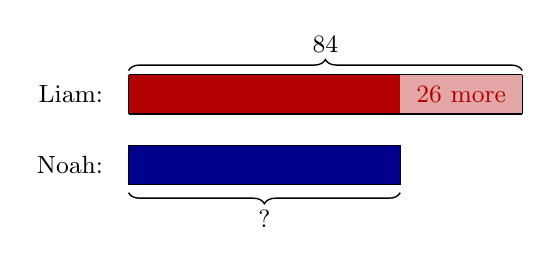
\begin{tikzpicture}[>=Stealth, baseline={(0,0.5)}]
    \node[anchor=east, font=\small] at (-0.2,1.2) {Liam:};
    \path[fill=redbar] (0,0.95) -- (3.45,0.95) -- (3.45,1.45) -- (0,1.45) -- cycle;
    \draw[black, line width=0.5pt] (0,0.95) -- (3.45,0.95);
    \draw[black, line width=0.5pt] (0,1.45) -- (3.45,1.45);
    \draw[black, line width=0.5pt] (0,0.95) -- (0,1.45);
    \fill[redbar, opacity=0.35] (3.45,0.95) rectangle (5.0,1.45);
    \draw[black, line width=0.5pt] (3.45,0.95) -- (5.0,0.95);
    \draw[black, line width=0.5pt] (3.45,1.45) -- (5.0,1.45);
    \draw[black, line width=0.5pt] (5.0,0.95) -- (5.0,1.45);
    \node[font=\small, text=redbar] at (4.225,1.2) {26 more};
    \topbrace{0}{5.0}{1.5}{84}
    \node[anchor=east, font=\small] at (-0.2,0.3) {Noah:};
    \bbar{0}{3.45}{0.05}{bluebar}{}
    \botbrace{0}{3.45}{-0.05}{?}
  \end{tikzpicture}

  \vspace{0.6em}
  Equation: $\blank - \blank = \blank$

  % Repeated-Unit Model
  \item \textbf{Apples : oranges is $4:7$. There are 28 apples. How many oranges?}

  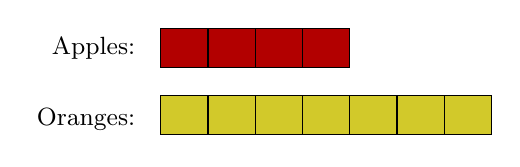
\begin{tikzpicture}[>=Stealth, baseline={(0,0.5)}]
    \node[anchor=east, font=\small] at (-0.2,0.9) {Apples:};
    \bbar{0}{2.4}{0.65}{redbar}{}
    \foreach \x in {0.6,1.2,1.8} { \draw (\x,0.65) -- (\x,1.15); }
    \node[anchor=east, font=\small] at (-0.2,0) {Oranges:};
    \bbar{0}{4.2}{-0.2}{yellowbar}{}
    \foreach \x in {0.6,1.2,1.8,2.4,3.0,3.6} { \draw (\x,-0.2) -- (\x,0.3); }
  \end{tikzpicture}

  \vspace{0.6em}
  1 unit $= 28 \div 4 = \blank[1.2cm]$ \hspace{2cm} Oranges $= 7 \times \blank[1.2cm] = \blank$
\end{questions}

\pagebreak

% =====================================================================
%  PART 4 -- Mental Math Strategies
% =====================================================================
\section*{Part 4: Mental Math Strategies (Friendly Numbers, Compensation \& Shifting)}

\noindent\textbf{Example 1 (Compatible Numbers):} Solve \textbf{$128 + 245 + 273 + 155 + 27 + 72$} by grouping friendly pairs.
\vspace{0.4em}

\begin{steps}
  \item[\stepnum{1}{p4s1}] \textbf{Identify compatible pairs}\\[0.2em]
  Look at the ones and tens digits to pair numbers that make whole hundreds:
  \\[0.4em]
  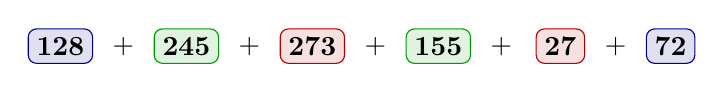
\begin{tikzpicture}[baseline={(0,0.1)}]
    \node[draw=bluebar, fill=bluebar!12, rounded corners=3pt, inner sep=3pt, font=\bfseries] at (0,0) {128};
    \node at (0.8,0) {+};
    \node[draw=greenbar, fill=greenbar!12, rounded corners=3pt, inner sep=3pt, font=\bfseries] at (1.6,0) {245};
    \node at (2.4,0) {+};
    \node[draw=redbar, fill=redbar!12, rounded corners=3pt, inner sep=3pt, font=\bfseries] at (3.2,0) {273};
    \node at (4.0,0) {+};
    \node[draw=greenbar, fill=greenbar!12, rounded corners=3pt, inner sep=3pt, font=\bfseries] at (4.8,0) {155};
    \node at (5.6,0) {+};
    \node[draw=redbar, fill=redbar!12, rounded corners=3pt, inner sep=3pt, font=\bfseries] at (6.35,0) {27};
    \node at (7.05,0) {+};
    \node[draw=bluebar, fill=bluebar!12, rounded corners=3pt, inner sep=3pt, font=\bfseries] at (7.75,0) {72};
  \end{tikzpicture}
  \vspace{0.3em}

  \item[\stepnum{2}{p4s2}] \textbf{Rearrange and group the pairs}\\[0.2em]
  \[ (128 + 72) + (245 + 155) + (273 + 27) \]

  \item[\stepnum{3}{p4s3}] \textbf{Add the friendly round hundreds}\\[0.2em]
  \[ 200 + 400 + 300 = \mathbf{900} \]
\end{steps}
\stepchain{p4s1,p4s2,p4s3}

\vspace{0.4em}
\noindent\textbf{Example 2 (Rounding \& Compensation):} Solve \textbf{$999 + 99 + 9$} using friendly benchmark numbers.
\vspace{0.4em}

\begin{steps}
  \item[\stepnum{1}{p4b1}] \textbf{Round up to the nearest powers of 10}\\[0.2em]
  Each number is just $1$ less than a round benchmark ($1000, 100, 10$):
  \\[0.4em]
  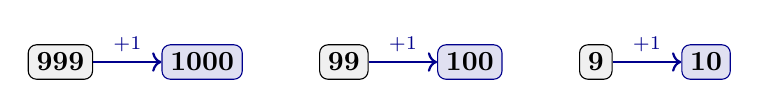
\begin{tikzpicture}[baseline={(0,0.1)}]
    \node[draw=black, fill=subtext!10, rounded corners=3pt, inner sep=3pt] (c1) at (0,0) {\textbf{999}};
    \node (b1) at (1.8,0) [draw=bluebar, fill=bluebar!12, rounded corners=3pt, inner sep=3pt] {\textbf{1000}};
    \draw[->, thick, bluebar] (c1) -- node[above, font=\scriptsize\bfseries] {$+1$} (b1);

    \node[draw=black, fill=subtext!10, rounded corners=3pt, inner sep=3pt] (c2) at (3.6,0) {\textbf{99}};
    \node (b2) at (5.2,0) [draw=bluebar, fill=bluebar!12, rounded corners=3pt, inner sep=3pt] {\textbf{100}};
    \draw[->, thick, bluebar] (c2) -- node[above, font=\scriptsize\bfseries] {$+1$} (b2);

    \node[draw=black, fill=subtext!10, rounded corners=3pt, inner sep=3pt] (c3) at (6.8,0) {\textbf{9}};
    \node (b3) at (8.2,0) [draw=bluebar, fill=bluebar!12, rounded corners=3pt, inner sep=3pt] {\textbf{10}};
    \draw[->, thick, bluebar] (c3) -- node[above, font=\scriptsize\bfseries] {$+1$} (b3);
  \end{tikzpicture}
  \vspace{0.3em}

  \item[\stepnum{2}{p4b2}] \textbf{Add the round numbers and track the total excess}\\[0.2em]
  We added $1 + 1 + 1 = 3$ extra, so we subtract $3$ from the round total:
  \[ (1000 + 100 + 10) - 3 = 1110 - 3 \]

  \item[\stepnum{3}{p4b3}] \textbf{Calculate the final sum}\\[0.2em]
  \[ 1110 - 3 = \mathbf{1107} \]
\end{steps}
\stepchain{p4b1,p4b2,p4b3}

\vspace{0.4em}
\noindent\textbf{Example 3 (The Shifting Method for Subtraction):} Solve \textbf{$900 - 396$} by shifting to a round number.
\vspace{0.4em}

\begin{steps}
  \item[\stepnum{1}{p4c1}] \textbf{Identify the nearest round hundred}\\[0.2em]
  $396$ is only $4$ away from $400$.
  \vspace{0.2em}

  \item[\stepnum{2}{p4c2}] \textbf{Add the same amount ($+4$) to both numbers}\\[0.2em]
  Adding the same number to both terms preserves the difference (no borrowing across zeroes!):
  \\[0.4em]
  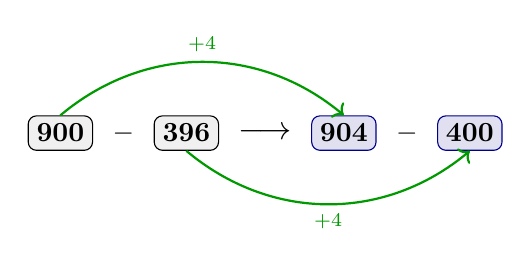
\begin{tikzpicture}[baseline={(0,0.15)}]
    \node[draw=black, fill=subtext!10, rounded corners=3pt, inner sep=3pt] (s1) at (0,0.3) {\textbf{900}};
    \node at (0.8,0.3) {$-$};
    \node[draw=black, fill=subtext!10, rounded corners=3pt, inner sep=3pt] (s2) at (1.6,0.3) {\textbf{396}};

    \node at (2.6,0.3) {\large $\longrightarrow$};

    \node[draw=bluebar, fill=bluebar!12, rounded corners=3pt, inner sep=3pt] (t1) at (3.6,0.3) {\textbf{904}};
    \node at (4.4,0.3) {$-$};
    \node[draw=bluebar, fill=bluebar!12, rounded corners=3pt, inner sep=3pt] (t2) at (5.2,0.3) {\textbf{400}};

    \draw[->, thick, greenbar] (s1.north) to[out=40, in=140] node[above, font=\scriptsize\bfseries, text=greenbar] {$+4$} (t1.north);
    \draw[->, thick, greenbar] (s2.south) to[out=-40, in=-140] node[below, font=\scriptsize\bfseries, text=greenbar] {$+4$} (t2.south);
  \end{tikzpicture}
  \vspace{0.3em}

  \item[\stepnum{3}{p4c3}] \textbf{Subtract without regrouping}\\[0.2em]
  \[ 900 - 396 = 904 - 400 = \mathbf{504} \]
\end{steps}
\stepchain{p4c1,p4c2,p4c3}

\pagebreak

\practicehead{Practice Questions}

\begin{questions}
  % Question 1: 4-term compatible pairs
  \item \textbf{Pair compatible numbers to make hundreds, then solve:}

  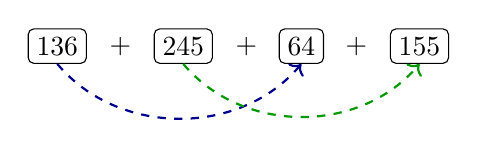
\begin{tikzpicture}[baseline={(0,0.1)}]
    \node[draw=black, rounded corners=2pt, inner sep=3pt] (q1) at (0,0) {136};
    \node at (0.8,0) {+};
    \node[draw=black, rounded corners=2pt, inner sep=3pt] (q2) at (1.6,0) {245};
    \node at (2.4,0) {+};
    \node[draw=black, rounded corners=2pt, inner sep=3pt] (q3) at (3.1,0) {64};
    \node at (3.8,0) {+};
    \node[draw=black, rounded corners=2pt, inner sep=3pt] (q4) at (4.6,0) {155};
    \draw[dashed, bluebar, thick, ->] (q1.south) to[out=-50, in=-130] (q3.south);
    \draw[dashed, greenbar, thick, ->] (q2.south) to[out=-50, in=-130] (q4.south);
  \end{tikzpicture}

  \vspace{0.4em}
  Equation: $(\blank + \blank) + (\blank + \blank) = \blank + \blank = \blank$

  % Question 2: 6-term compatible pairs
  \item \textbf{Rearrange into three compatible pairs to solve $118 + 265 + 234 + 135 + 66 + 82$:}

  \vspace{0.4em}
  Equation: $(\blank + \blank) + (\blank + \blank) + (\blank + \blank) = \blank + \blank + \blank = \blank$

  % Question 3: Compensation with 9s
  \item \textbf{Use rounding and compensation to calculate $499 + 199 + 19$:}

  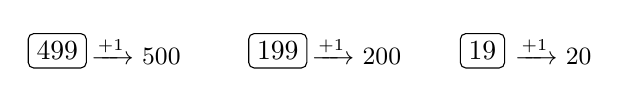
\begin{tikzpicture}[baseline={(0,0.1)}]
    \node[draw=black, rounded corners=2pt, inner sep=3pt] at (0,0) {499};
    \node at (1.0,0) [font=\small] {$\xrightarrow{+1}$ 500};
    \node[draw=black, rounded corners=2pt, inner sep=3pt] at (2.8,0) {199};
    \node at (3.8,0) [font=\small] {$\xrightarrow{+1}$ 200};
    \node[draw=black, rounded corners=2pt, inner sep=3pt] at (5.4,0) {19};
    \node at (6.3,0) [font=\small] {$\xrightarrow{+1}$ 20};
  \end{tikzpicture}

  \vspace{0.4em}
  Equation: $(\blank + \blank + \blank) - \blank = \blank - \blank = \blank$

  % Question 4: Shifting Method Subtraction
  \item \textbf{Use the shifting method (constant difference) to make a round subtrahend:}

  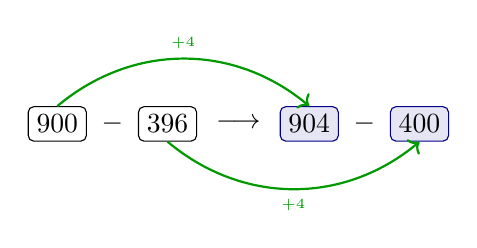
\begin{tikzpicture}[baseline={(0,0.1)}]
    \node[draw=black, rounded corners=2pt, inner sep=3pt] (sh1) at (0,0.2) {900};
    \node at (0.7,0.2) {$-$};
    \node[draw=black, rounded corners=2pt, inner sep=3pt] (sh2) at (1.4,0.2) {396};
    \node at (2.3,0.2) {$\longrightarrow$};
    \node[draw=bluebar, fill=bluebar!10, rounded corners=2pt, inner sep=3pt] (th1) at (3.2,0.2) {904};
    \node at (3.9,0.2) {$-$};
    \node[draw=bluebar, fill=bluebar!10, rounded corners=2pt, inner sep=3pt] (th2) at (4.6,0.2) {400};
    \draw[->, thick, greenbar] (sh1.north) to[out=40, in=140] node[above, font=\tiny\bfseries, text=greenbar] {$+4$} (th1.north);
    \draw[->, thick, greenbar] (sh2.south) to[out=-40, in=-140] node[below, font=\tiny\bfseries, text=greenbar] {$+4$} (th2.south);
  \end{tikzpicture}

  \vspace{0.4em}
  \begin{enumerate}[label=(\alph*), itemsep=0.8em, leftmargin=1.5em]
    \item $900 - 396 = (\blank + 4) - (396 + 4) = 904 - 400 = \blank$
    \item $800 - 297 = (800 + \blank) - (297 + \blank) = \blank - 300 = \blank$
    \item $600 - 189 = (600 + \blank) - (189 + \blank) = \blank - \blank = \blank$
    \item $1000 - 495 = (1000 + \blank) - (495 + \blank) = \blank - 500 = \blank$
  \end{enumerate}
\end{questions}
\end{document}